% Name: Half adder
% Description: An XOR gate for the sum and an AND gate for the carry, with TikZ's US-style logic symbols.
% Tags: half adder, logic gates, XOR, arithmetic circuit

\usetikzlibrary{circuits.logic.US}

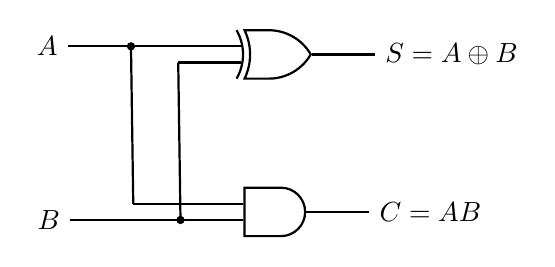
\begin{tikzpicture}[circuit logic US, thick, every circuit symbol/.style={thick}]
  \node[xor gate] (sum) at (3,1) {};
  \node[and gate] (carry) at (3,-1) {};

  \draw (sum.input 1) -- ++(left:14mm) coordinate (a1);
  \draw (carry.input 1) -- ++(left:14mm) coordinate (a2);
  \draw (sum.input 2) -- ++(left:8mm) coordinate (b1);
  \draw (carry.input 2) -- ++(left:8mm) coordinate (b2);
  \draw (a1) -- (a2) (b1) -- (b2);
  \draw (a1) -- ++(left:8mm) node[left] {$A$};
  \draw (b2) -- ++(left:14mm) node[left] {$B$};
  \fill (a1) circle (1.5pt) (b2) circle (1.5pt);

  \draw (sum.output) -- ++(right:8mm) node[right] {$S = A \oplus B$};
  \draw (carry.output) -- ++(right:8mm) node[right] {$C = AB$};
\end{tikzpicture}
